%% \documentclass[addpoints]{exam}
\documentclass[addpoints,answers]{exam}
\usepackage{amsmath,amsthm,amssymb,mathdots}
% \usepackage{fourier}
% \usepackage{courier}
%% \usepackage{fontspec}
%% \usepackage{euler}
%% \usepackage[utf8]{inputenc} % Required for inputting international characters
%% \usepackage[T1]{fontenc} % Output font encoding for international characters
%% \usepackage{mathpazo} % Use the Palatino font
\usepackage{graphicx} % Required for including images
\usepackage{booktabs} % Required for better horizontal rules in tables
\usepackage{enumerate} % To modify the enumerate environment

\usepackage{multicol}
\usepackage{multirow}
\usepackage{subfigure}
%\usepackage[most]{tcolorbox}
\newcounter{testexample}
\usepackage{xparse}
\usepackage{lipsum}
\usepackage[UTF8,noindent]{ctex}
\usepackage{extarrows}
\usepackage{animate}
\usepackage{dcolumn}
\usepackage{pgf}
\usepackage{tikz}
\usetikzlibrary{calc}
\usetikzlibrary{arrows,snakes,backgrounds,shapes,patterns,fit}
\usetikzlibrary{matrix,fit,positioning,decorations.pathmorphing}
\usetikzlibrary{shapes.geometric}


\usepackage{listings}
\lstset{
        language=c,
        keywordstyle=\color{red},
        %% frame=single,
        basicstyle=\ttfamily,
        commentstyle=\color{blue},
        breakindent=0pt,
        rulesepcolor=\color{red!20!green!20!blue!20},
        rulecolor=\color{black},
        tabsize=4,
        numbersep=5pt,
        breaklines=true,
        % backgroundcolor=\color{red!15},
        showstringspaces=false,
        showspaces=false,
        showtabs=false,
        extendedchars=false,
        escapeinside=``,
}

\usepackage{refcount}
\usepackage{multicol}
\newcounter{countitems}
\newcounter{nextitemizecount}
\newcommand{\setupcountitems}{%
        \stepcounter{nextitemizecount}%
        \setcounter{countitems}{0}%
        \preto\item{\stepcounter{countitems}}%
}
\makeatletter
\newcommand{\computecountitems}{%
        \edef\@currentlabel{\number\c@countitems}%
        \label{countitems@\number\numexpr\value{nextitemizecount}-1\relax}%
}
\newcommand{\nextitemizecount}{%
        \getrefnumber{countitems@\number\c@nextitemizecount}%
}
\newcommand{\previtemizecount}{%
        \getrefnumber{countitems@\number\numexpr\value{nextitemizecount}-1\relax}%
}
\makeatother    
\newenvironment{AutoMultiColItemize}{%
        \ifnumcomp{\nextitemizecount}{>}{3}{\begin{multicols}{2}}{}%
                \setupcountitems\begin{itemize}}%
                {\end{itemize}%
                \unskip\computecountitems\ifnumcomp{\previtemizecount}{>}{3}{\end{multicols}}{}}

\tikzset{mystyle/.style n args={5}{
    rectangle,
    draw,
    fill=#1!50,
    % rounded corners,
    minimum height=#2cm,
    minimum width=#3cm,
    text width=#4cm,
    align=#5
  }}

\tikzset{mystyle2/.style n args={5}{
    rectangle,
    % draw,
    fill=#1!30,
    % rounded corners,
    minimum height=#2,
    minimum width=#3\textwidth,
    text width=#4\textwidth,
    align=#5,
    inner sep=0,
  }}

\tikzset{myarrow/.style n args={2}{
    ->,
    #1,
    line width=#2
  }}


% ######### DEFINE COLOR ###############
\definecolor{blue}{rgb}{0.0,0.0,1.0}
\definecolor{red}{rgb}{1.0,0.0,0.0}
\definecolor{purple}{rgb}{0.75, 0.0, 1.0}

\def\blue{\textcolor{blue}}
\def\red{\textcolor{red}}
\def\purple{\textcolor{purple}}

\def\tf{\ttfamily}
\def\lst{\lstinline}
\def\ds{\displaystyle}
\def\cd{\cdots}
\def\dd{\ddots}
\def\vd{\vdots}
\def\id{\iddots}
\def\ft{\frametitle}
\def\diag{\mathrm{diag}}
\def\Im{\mathrm{Im~}}
\def\Ker{\mathrm{Ker~}}
\def\R{\mathbb R}
\def\C{\mathbb C}
\def\cov{\mathrm{cov}}
\def\E{\mathbb E}
\def\var{\mathrm{var}}
\def\dim{\mathrm{dim~}}
\def\rank{\mathrm{r}}
\def\tr{\mathrm{tr}}
\def\det{\mathrm{det}}
\def\H{{\mathrm{H}}}
\def\I{{\mathrm{I}}}
\def\ML{{\mathrm{ML}}}
\def\MLE{{\mathrm{MLE}}}
\def\MAP{{\mathrm{MAP}}}
\def\Bern{\mathrm{Bern}}
\def\Beta{\mathrm{Beta}}
\def\KL{\mathrm{KL}}
\def\const{\mathrm{const}}
\newcommand{\ttt}[1]{\texttt{#1}}

\def\cA{\mathcal{A}}
\def\cB{\mathcal{B}}
\def\cC{\mathcal{C}}
\def\cD{\mathcal{D}}
\def\cE{\mathcal{E}}
\def\cF{\mathcal{F}}
\def\cG{\mathcal{G}}
\def\cH{\mathcal{H}}
\def\cI{\mathcal{I}}
\def\cJ{\mathcal{J}}
\def\cK{\mathcal{K}}
\def\cL{\mathcal{L}}
\def\cM{\mathcal{M}}
\def\cN{\mathcal{N}}
\def\cO{\mathcal{O}}
\def\cP{\mathcal{P}}
\def\cQ{\mathcal{Q}}
\def\cR{\mathcal{R}}
\def\cS{\mathcal{S}}
\def\cT{\mathcal{T}}
\def\cU{\mathcal{U}}
\def\cV{\mathcal{V}}
\def\cW{\mathcal{W}}
\def\cX{\mathcal{X}}
\def\cY{\mathcal{Y}}
\def\cZ{\mathcal{Z}}

\def\bA{{\mathbf{A}}}
\def\bB{{\mathbf{B}}}
\def\bC{{\mathbf{C}}}
\def\bD{{\mathbf{D}}}
\def\bE{{\mathbf{E}}}
\def\bF{{\mathbf{F}}}
\def\bG{{\mathbf{G}}}
\def\bH{{\mathbf{H}}}
\def\bI{{\mathbf{I}}}
\def\bJ{{\mathbf{J}}}
\def\bK{{\mathbf{K}}}
\def\bL{{\mathbf{L}}}
\def\bM{{\mathbf{M}}}
\def\bN{{\mathbf{N}}}
\def\bO{{\mathbf{O}}}
\def\bP{{\mathbf{P}}}
\def\bQ{{\mathbf{Q}}}
\def\bR{{\mathbf{R}}}
\def\bS{{\mathbf{S}}}
\def\bT{{\mathbf{T}}}
\def\bU{{\mathbf{U}}}
\def\bV{{\mathbf{V}}}
\def\bW{{\mathbf{W}}}
\def\bX{{\mathbf{X}}}
\def\bY{{\mathbf{Y}}}
\def\bZ{{\mathbf{Z}}}

\def\vA{\boldsymbol{A}}
\def\vB{\boldsymbol{B}}
\def\vC{\boldsymbol{C}}
\def\vD{\boldsymbol{D}}
\def\vE{\boldsymbol{E}}
\def\vF{\boldsymbol{F}}
\def\vG{\boldsymbol{G}}
\def\vH{\boldsymbol{H}}
\def\vI{\boldsymbol{I}}
\def\vJ{\boldsymbol{J}}
\def\vK{\boldsymbol{K}}
\def\vL{\boldsymbol{L}}
\def\vM{\boldsymbol{M}}
\def\vN{\boldsymbol{N}}
\def\vO{\boldsymbol{O}}
\def\vP{\boldsymbol{P}}
\def\vQ{\boldsymbol{Q}}
\def\vR{\boldsymbol{R}}
\def\vS{\boldsymbol{S}}
\def\vT{\boldsymbol{T}}
\def\vU{\boldsymbol{U}}
\def\vV{\boldsymbol{V}}
\def\vW{\boldsymbol{W}}
\def\vX{\boldsymbol{X}}
\def\vY{\boldsymbol{Y}}
\def\vZ{\boldsymbol{Z}}

\def\v0{{\boldsymbol{0}}}
\def\va{{\boldsymbol{a}}}
\def\vb{{\boldsymbol{b}}}
\def\vc{{\boldsymbol{c}}}
\def\vd{{\boldsymbol{d}}}
\def\ve{{\boldsymbol{e}}}
\def\vf{{\boldsymbol{f}}}
\def\vg{{\boldsymbol{g}}}
\def\vh{{\boldsymbol{h}}}
\def\vi{{\boldsymbol{i}}}
\def\vj{{\boldsymbol{j}}}
\def\vk{{\boldsymbol{k}}}
\def\vl{{\boldsymbol{l}}}
\def\vm{{\boldsymbol{m}}}
\def\vn{{\boldsymbol{n}}}
\def\vo{{\boldsymbol{o}}}
\def\vp{{\boldsymbol{p}}}
\def\vq{{\boldsymbol{q}}}
\def\vr{{\boldsymbol{r}}}
\def\vs{{\boldsymbol{s}}}
\def\vt{{\boldsymbol{t}}}
\def\vu{{\boldsymbol{u}}}
\def\vv{{\boldsymbol{v}}}
\def\vw{{\boldsymbol{w}}}
\def\vx{{\boldsymbol{x}}}
\def\vy{{\boldsymbol{y}}}
\def\vz{{\boldsymbol{z}}}

\def\ba{{\mathbf{a}}}
\def\bb{{\mathbf{b}}}
\def\bc{{\mathbf{c}}}
\def\bd{{\mathbf{d}}}
\def\be{{\mathbf{e}}}
\def\bf{{\mathbf{f}}}
\def\bg{{\mathbf{g}}}
\def\bh{{\mathbf{h}}}
\def\bi{{\mathbf{i}}}
\def\bj{{\mathbf{j}}}
\def\bk{{\mathbf{k}}}
\def\bl{{\mathbf{l}}}
\def\bm{{\mathbf{m}}}
\def\bn{{\mathbf{n}}}
\def\bo{{\mathbf{o}}}
\def\bp{{\mathbf{p}}}
\def\bq{{\mathbf{q}}}
\def\br{{\mathbf{r}}}
\def\bs{{\mathbf{s}}}
\def\bt{{\mathbf{t}}}
\def\bu{{\mathbf{u}}}
\def\bv{{\mathbf{v}}}
\def\bw{{\mathbf{w}}}
\def\bx{{\mathbf{x}}}
\def\by{{\mathbf{y}}}
\def\bz{{\mathbf{z}}}


\def\valpha{\boldsymbol{\alpha}}
\def\vbeta{\boldsymbol{\beta}}
\def\vgamma{\boldsymbol{\gamma}}
\def\vxi{\boldsymbol{\xi}}
\def\vzeta{\boldsymbol{\zeta}}
\def\veta{\boldsymbol{\eta}}
\def\vepsilon{\boldsymbol{\epsilon}}
\def\vphi{\boldsymbol{\phi}}
\def\vvarphi{\boldsymbol{\varphi}}
\def\vsigma{\boldsymbol{\sigma}}
\def\vomega{\boldsymbol{\omega}}
\def\vtau{\boldsymbol{\tau}}
\def\vmu{\boldsymbol{\mu}}

\def\vLambda{\boldsymbol{\Lambda}}
\def\vSigma{\boldsymbol{\Sigma}}
\def\vTheta{{\boldsymbol{\Theta}}}
\def\vtheta{\boldsymbol{\theta}}

\renewcommand{\proofname}{\textbf{证明}}
\newtheorem{li}{例}%[section]
%\newtheorem*{li*}{例}
\newtheorem{lianxi}{练习}
\newtheorem*{jielun}{结论}
\newtheorem*{dingli}{定理}
\newtheorem*{mingti}{{命题}} 
\newtheorem*{yinli}{{引理}} 
\newtheorem*{tuilun}{{推论}}
\newtheorem*{dingyi}{{定义}}
\newtheorem*{biancheng}{{编程}}
\newtheorem*{jie}{{解}}
\newtheorem{zhu}{{注}}
\newtheorem*{xingzhi}{{性质}}%[subsection]
\newtheorem*{wenti}{{问题}}
\newtheorem*{rem}{{Remark}}
\newtheorem*{lem}{{Lemma}}
\newtheorem*{remark}{{注}}
\def\exampletext{知识点回顾} % If English
\NewDocumentEnvironment{testexample}{ O{} }
{
\colorlet{colexam}{red!55!black} % Global example color
\newtcolorbox[use counter=testexample]{testexamplebox}{%
    % Example Frame Start
    empty,% Empty previously set parameters
    title={\exampletext: #1},% use \thetcbcounter to access the testexample counter text
    % Attaching a box requires an overlay
    attach boxed title to top left,
       % Ensures proper line breaking in longer titles
       minipage boxed title,
    % (boxed title style requires an overlay)
    boxed title style={empty,size=minimal,toprule=0pt,top=4pt,left=3mm,overlay={}},
    coltitle=colexam,fonttitle=\bfseries,
    before=\par\medskip\noindent,parbox=false,boxsep=0pt,left=3mm,right=0mm,top=2pt,breakable,pad at break=0mm,
       before upper=\csname @totalleftmargin\endcsname0pt, % Use instead of parbox=true. This ensures parskip is inherited by box.
    % Handles box when it exists on one page only
    overlay unbroken={\draw[colexam,line width=.5pt] ([xshift=-0pt]title.north west) -- ([xshift=-0pt]frame.south west); },
    % Handles multipage box: first page
    overlay first={\draw[colexam,line width=.5pt] ([xshift=-0pt]title.north west) -- ([xshift=-0pt]frame.south west); },
    % Handles multipage box: middle page
    overlay middle={\draw[colexam,line width=.5pt] ([xshift=-0pt]frame.north west) -- ([xshift=-0pt]frame.south west); },
    % Handles multipage box: last page
    overlay last={\draw[colexam,line width=.5pt] ([xshift=-0pt]frame.north west) -- ([xshift=-0pt]frame.south west); },%
    }
\begin{testexamplebox}}
{\end{testexamplebox}\endlist}

\usepackage[utf8]{inputenc}
\usepackage{geometry}
\usepackage{graphicx}
\geometry{left=20mm,right=20mm,top=20mm,bottom=20mm}
\DeclareMathOperator{\sech}{sech}

\begin{document}

\begin{center}
  \fbox{\fbox{\parbox{5.5in}{\centering
        2020-2021学年第二学期数学实验\\
        实验报告\\
  }}} 
\end{center}

\vspace{5mm}

\begin{center}
  \makebox[0.3\textwidth]{姓名:\enspace\hrulefill}
  \hspace{5mm}
  \makebox[0.3\textwidth]{学号:\enspace\hrulefill}
  \hspace{5mm}
  \makebox[0.3\textwidth]{截止日期:\enspace2021.6.25}
\end{center}

\pointname{分}
\renewcommand{\solutiontitle}{\noindent\textbf{解:}\enspace}
%%%%%%%%%%%%%%%%%%%%%%%%%%%%%%%%%%%%%%%%%%%%%%%%%%%%%%%%%%%%%%%%%%%%%%%%%%%%%%%%

%% \begin{center}
%%   \hqword{题号}
%%   \hpword{分值}
%%   \htword{总分}
%%   \hsword{得分}
%%   \cellwidth{2.2em}
%%   \gradetable[h][questions]
%% \end{center}

\begin{remark}
	本报告分为两部分内容,即
	\begin{itemize}
		\item 利用神经网络求解偏微分方程(三选一)
		\item 利用LSTM预测金融市场(必选)
	\end{itemize}

实验内容应包括:
\begin{itemize}
	\item 数据处理 
	\item 网络架构
	\item 网络参数(包括网络层数、每层的神经元个数等)对训练的影响
	\item 尽可能给出可视化结果, 包括相关结果的图像
	\item 尽可能把报告内容写得丰富一些,这可以自由发挥
	\item 建议大家编译latex文件时,安装Ctex+TexStudio。
	\item 最终的报告中,请把无关部分注释掉。
\end{itemize}
\end{remark}

\section{利用神经网络求解偏微分方程}
   \subsection{Schr\"odinger方程} 利用神经网络PINN求解一维非线性Schrodinger方程  
  \begin{subequations}\label{eq:Schrodinger}
    \begin{align}
      i h_t + 0.5 h_{xx} + |h|^2h = 0, & \quad  x\in[-5,5],   t\in (0,\pi/2], \label{eq:schrodinger_ODE}\\
        h(0,x) = 2 \sech (x), & \quad x \in [-5,5] & \label{eq:schrodinger_IC}\\
        h(t,-5) = h(t, 5), & \quad t\in (0,\pi/2] \label{eq:schrodinger_BC1}\\
          h_x(t,-5) = h_x(t, 5), & \quad t\in (0,\pi/2] \label{eq:schrodinger_BC2}
    \end{align}
  \end{subequations}
  其中$i$为虚数符号,$h(x,t) = u(x,t) + i v(x,t)$为复值函数,\eqref{eq:schrodinger_BC1}和\eqref{eq:schrodinger_BC2}为周期边界条件,$\sech$为双曲正弦函数,即
  $$
  \sech x = \frac{2}{e^x + e^{-x}}.
  $$
  \eqref{eq:Schrodinger}可改写为$u$和$v$的偏微分方程组
  \begin{subequations}\label{eq:Schrodinger_uv}
    \begin{align}
      u_t + 0.5 v_{xx} + (u^2+v^2)v = 0,  & \quad  x\in[-5,5],   t\in (0,\pi/2], \label{eq:schrodinger_ODE_u}\\
        v_t - 0.5 u_{xx} - (u^2+v^2)u = 0, & \quad  x\in[-5,5],   t\in (0,\pi/2], \label{eq:schrodinger_ODE_v}\\
          u(0,x) = 2 \sech (x), & \quad x \in [-5,5] & \label{eq:schrodinger_IC_u}\\
          v(0,x) = 0, & \quad x \in [-5,5] & \label{eq:schrodinger_IC_v}\\
          u(t,-5) = u(t, 5), & \quad t\in (0,\pi/2] \label{eq:schrodinger_BC1_u}\\
            v(t,-5) = v(t, 5), & \quad t\in (0,\pi/2] \label{eq:schrodinger_BC1_v}\\
              u_x(t,-5) = u_x(t, 5), & \quad t\in (0,\pi/2] \label{eq:schrodinger_BC2_u}\\
               v_x(t,-5) = v_x(t, 5), & \quad t\in (0,\pi/2] \label{eq:schrodinger_BC2_v}
    \end{align}
  \end{subequations}

  \begin{remark}
    薛定谔方程是一个经典的场方程,用于研究量子力学系统,包括非线性波在光纤和波导中的传播、玻色-爱因斯坦凝聚和等离子体波。在光学中,非线性项来自于给定材料的与强度有关的折射率。类似地,玻色-爱因斯坦凝聚的非线性项是相互作用的多体系统的平均场相互作用的结果。
  \end{remark}

  \begin{figure}[htbp]
    \centering
    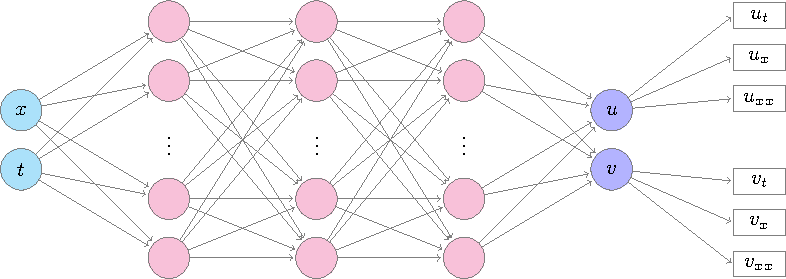
\includegraphics[width=5in]{tikz/Net1.pdf}
    \caption{求解薛定谔方程的神经网络架构}
  \end{figure}

 \paragraph{损失函数} 损失函数可表示为
    $$
    \cL(\vTheta) = \cL_{\mathrm{PDE}}(\vTheta) + \lambda_1 \cL_{\mathrm{IC}}(\vTheta) + \lambda_2 \cL_{\mathrm{BC}}(\vTheta)
    $$
    其中
    $$
    \begin{aligned}
      \cL_{\mathrm{PDE}}(\vTheta) = \frac1{N_{\mathrm{PDE}}} \sum_{n=1}^{N_{\mathrm{PDE}}} \left\{  \left[\hat u_t (t_n, x_n) + 0.5 \hat v_{xx}(t_n, x_n) + \left(\hat u(t_n, x_n)^2+\hat v(t_n, x_n)^2\right)\hat v(t_n, x_n) \right]^2 \right. \\
      \quad \left. + \left[\hat v_t(t_n, x_n) - 0.5 \hat u_{xx}(t_n, x_n) - \left(\hat u(t_n, x_n)^2+\hat v(t_n, x_n)^2\right)\hat u(t_n, x_n)\right]^2 \right\},
    \end{aligned}
    $$
    $$
    \begin{aligned}
      \cL_{\mathrm{IC}}(\vTheta) = \frac1{N_{\mathrm{IC}}} \sum_{n=1}^{N_{\mathrm{IC}}} \left\{\left[\hat u(0,x_n) - 2 \sech (x_n)\right]^2 + \hat v(0, x_n)^2 \right\}
    \end{aligned}
    $$
    $$
    \begin{aligned}
      \cL_{\mathrm{BC}}(\vTheta) = \frac1{N_{\mathrm{BC}}} \sum_{n=1}^{N_{\mathrm{BC}}} \left\{
      \left[\hat u(t_n,-5) - \hat u(t_n, 5)\right]^2 + 
      \left[\hat v(t_n,-5) - \hat v(t_n, 5)\right]^2 + \right. \\
      \quad \left. \left[\hat u_x(t_n,-5) - \hat u_x(t_n, 5)\right]^2 +
      \left[\hat v_x(t_n,-5) - \hat v_x(t_n, 5)\right]^2 
      \right\}
    \end{aligned}
    $$
    为方便, 这里用$\hat u$和$\hat v$表示网络的输出, 即
    $$
    \hat u(t, x) := u(t, x; \vTheta), ~~
    \hat u(t, x) := v(t, x; \vTheta).
    $$
   \subsection{网络结构搭建}
   \subsubsection{导入所需要的模块}
   (代码在最后)
   深度学习框架torch,
   优化计算.torch.optim,
   函数计算torch.nn,
   调参操作torch.optim.lr\_scheduler,
   处理文件和目录os,
   处理多维数组numpy,
   文件 文件夹读写操作shutil,
   绘图操作matplotlib.pyplot。
   \subsubsection{构建函数}
   其中包括:1.规定定义域,创建方程内函数,以及函数真值。2.调用函数示例
   \subsubsection{构建数据集}
   包括训练集的生成和测试集的生成
   \subsubsection{激活函数}
   可选择tanh, ReLU, LeakyReLU, sigmoid, softplus
   \subsubsection{计算网络输入,输出的梯度}
   compute the derivative of outputs associated with inputs.
   \subsubsection{搭建神经网络Network Archetecture}
   其中包括DNN: Deep Neural Network和 Residual DNN: Residual Deep Neural Network 和PINN: Physics Informed Neural Networks和Residual PINN: Residual Physics Informed Neural Networks
  
   \subsubsection{特殊条件处理} 我们从方程的定义出发,分别从实数和虚数两个角度考虑改写方程,同时也将初值条件加以替换:
   \begin{subequations}\label{eq:ac}
    \begin{gather*}
    h = u + iv\\
    - v_t + 0.5u_x x + (u^2 + v^2)u +i u_t + i(u^2  + v^2) = 0\\
    \end{gather*}    
    实数部分与虚数部分分别为0:
    \begin{gather*}
    - v_t + 0.5u_x x + (u^2 + v^2)u = 0\\
    u_t + u^2  + v^2 = 0\\
    \end{gather*}
  \end{subequations}
    在这里将初值条件设置为$$\mid h(0,x) \mid = 2sech(x)$$
    \subsubsection{训练过程及检验过程}
    接下来显示各种结果

   \subsection{不同网络训练结果之PiNN}
	网络参数选取为:dim\_hidden=50, hidden\_layers=4
	
	训练参数为:epochs\_Adam=5000, epochs\_LBFGS=200
	
	初始学习率和学习率改变速率为:lr=0.001, step\_size=2000, gamma=0.7
	
	训练用采样点: 使用Uniform Sampling方法采样20000个点, 其中x方向采样200个点, t方向采样100个时刻, 边界条件和初值条件使用Uniform Sampling方法采样400个点
	
	检验用采样点: 使用Uniform Sampling方法采样10000个点, 边界条件和初值条件使用Uniform Sampling方法采样400个点
	下面图片是训练的损失函数随训练Epoch的变化过程
	\clearpage
     \vspace{0.5cm}
    \begin{figure}
    	\centering
    	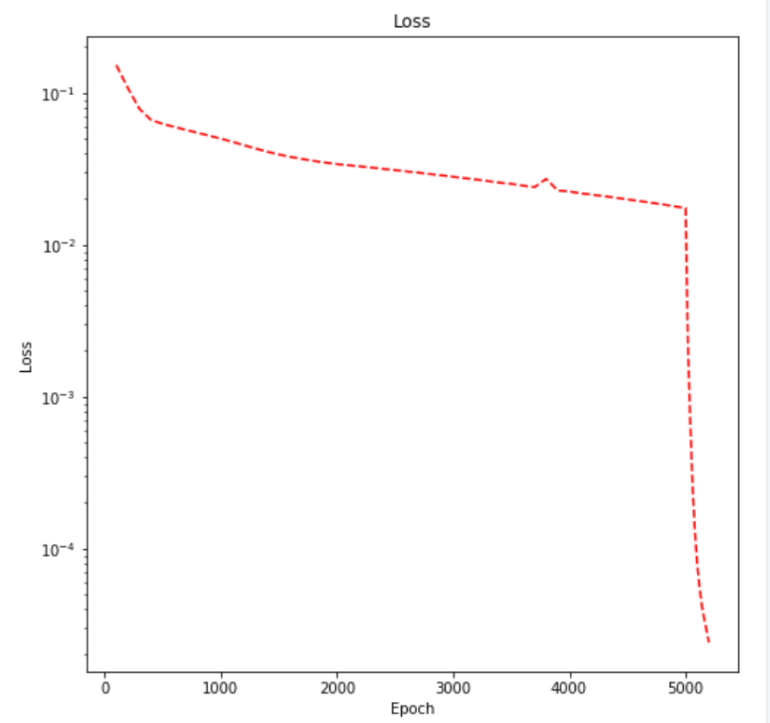
\includegraphics[height=4cm]{4.png}
    	\caption{Loss随Epoch增长之间的关系}
    \end{figure}
	测试用采样点: 使用Uniform Sampling方法采样256个点
	生成的数据由给定的参数 t 决定
	这里我们小组参照文章中的例子选取了t=0.59, 0.79, 0.98三个时刻来展示结果
	测试结果显示如下:
	\clearpage
    \vspace{0.5cm}
        \vspace{0.5cm}
    \begin{figure}
    	\centering
    	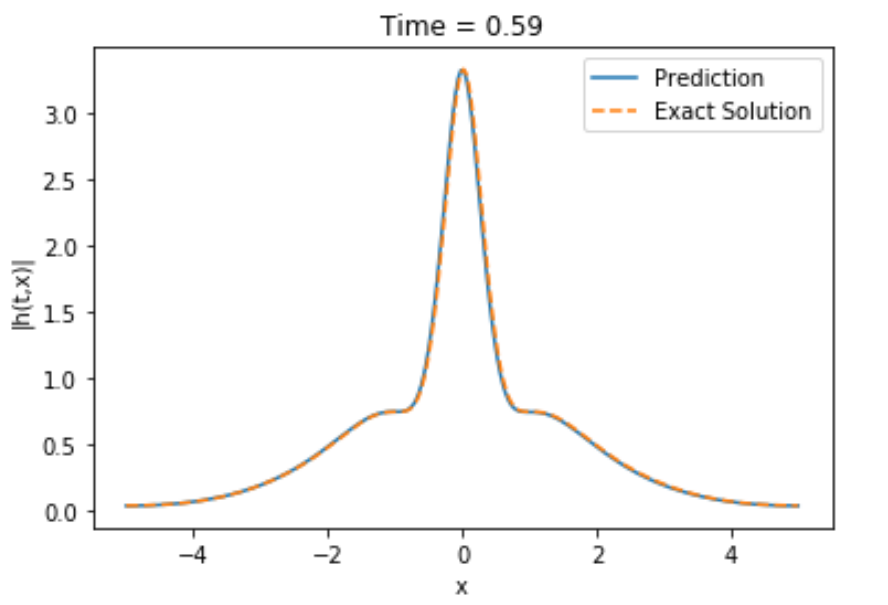
\includegraphics[height=4cm]{1.png}
    	\caption{t=0.59}
    \end{figure}
    
    \begin{figure}
    	\centering
    	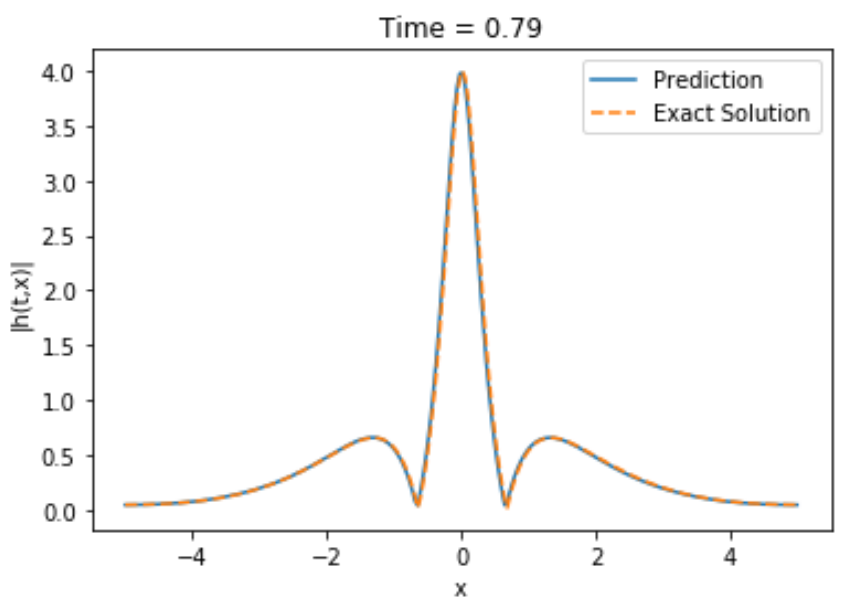
\includegraphics[height=4cm]{2.png}
    	\caption{t=0.79}
    \end{figure}
    
    \begin{figure}
    	\centering
    	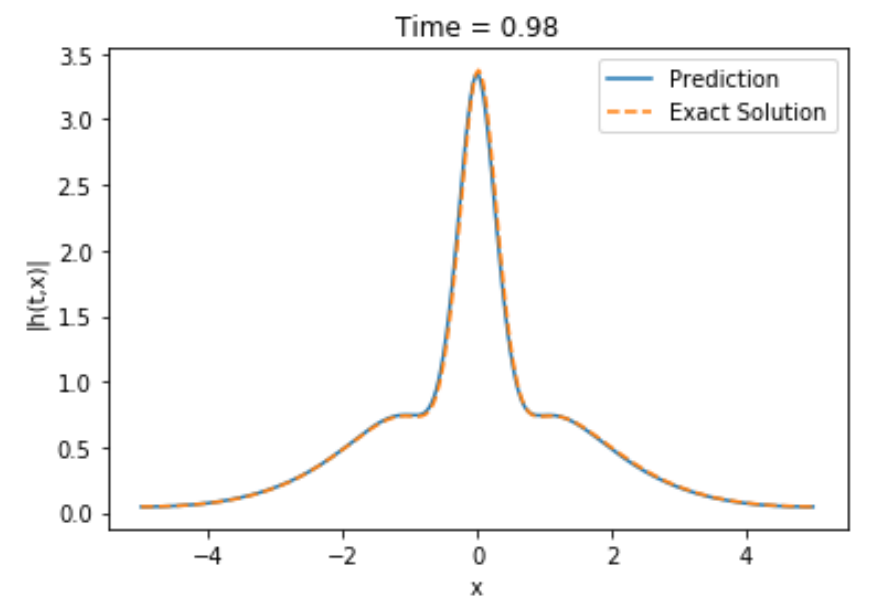
\includegraphics[height=4cm]{3.png}
    	\caption{t=0.98}
    \end{figure}
    
    \clearpage


   \subsection{不同网络训练结果之ResPiNN}
    
    网络参数选取为:dim\_hidden=50, hidden\_layers=4
    
    训练参数为:epochs\_Adam=5000, epochs\_LBFGS=200
    
    初始学习率和学习率改变速率为:lr=0.001, step\_size=2000, gamma=0.7
    
    训练用采样点: 使用Uniform Sampling方法采样20000个点, 其中x方向采样200个点, t方向采样100个时刻, 边界条件和初值条件使用Uniform Sampling方法采样400个点
    
    检验用采样点: 使用Uniform Sampling方法采样10000个点, 边界条件和初值条件使用Uniform Sampling方法采样400个点
    下面图片是训练的损失函数随训练Epoch的变化过程
    \clearpage
    \vspace{0.5cm}
    \begin{figure}
    	\centering
    	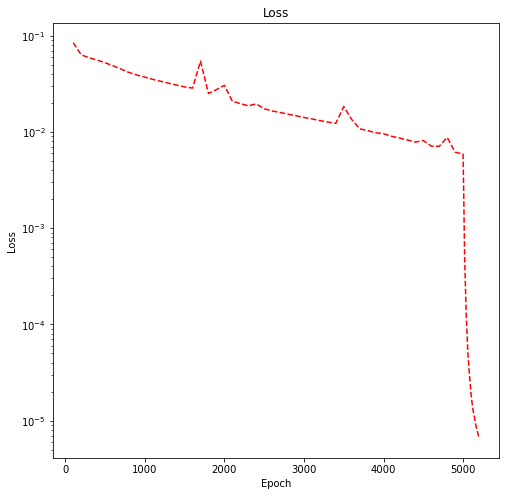
\includegraphics[height=8cm]{5.png}
    	\caption{Loss随Epoch增长之间的关系}
    \end{figure}
    
    
    
    测试用采样点: 使用Uniform Sampling方法采样256个点
    生成的数据由给定的参数 t 决定
    类似地我们选择t=0.59, 0.79, 0.98三个时刻来展示结果
    测试结果显示如下:
    \clearpage
    \vspace{0.5cm}
    \vspace{0.5cm}
    \begin{figure}
    	\centering
    	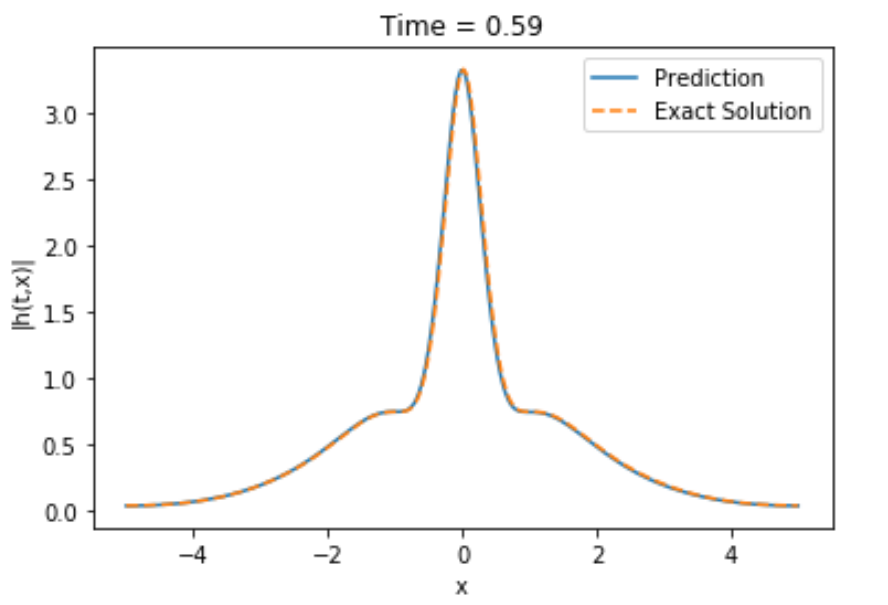
\includegraphics[height=4cm]{1.png}
    	\caption{t=0.59}
    \end{figure}
    
    \begin{figure}
    	\centering
    	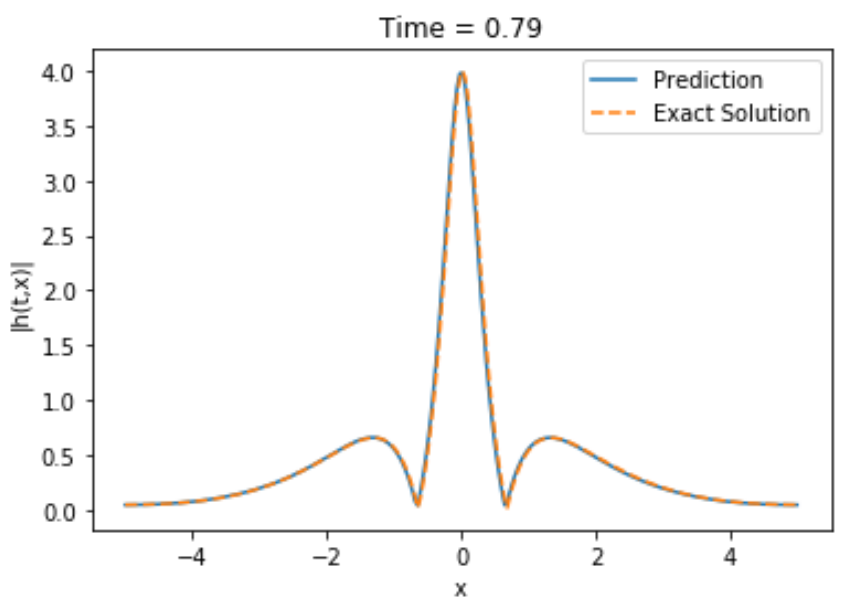
\includegraphics[height=4cm]{2.png}
    	\caption{t=0.79}
    \end{figure}
    
    \begin{figure}
    	\centering
    	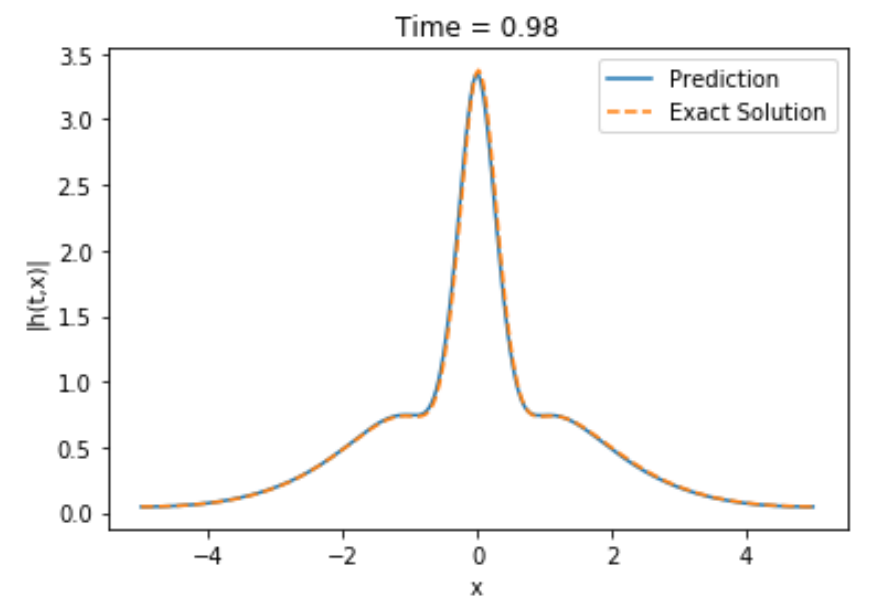
\includegraphics[height=4cm]{3.png}
    	\caption{t=0.98}
    \end{figure}
    
    \clearpage
   \subsection{两种网络的比较}
    通过比较结果可以知道两种网络预测得到的解基本一样:不仅损失函数变化差不多,图像也是类似的。
    接下来选取一个时间t=0.98来分析方程结果,并与精确解作对比:上面两个图像即是我们组的最终结果。
    \clearpage
    \begin{figure}
    	\centering
    	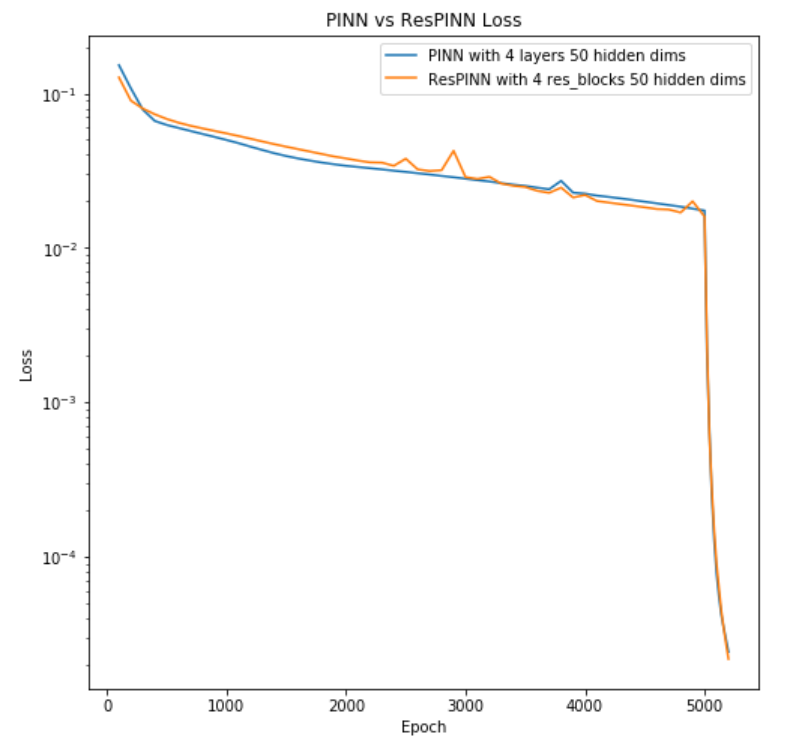
\includegraphics[height=4cm]{6.png}
    	\caption{Loss比较图}
    \end{figure}
    
    \begin{figure}
    	\centering
    	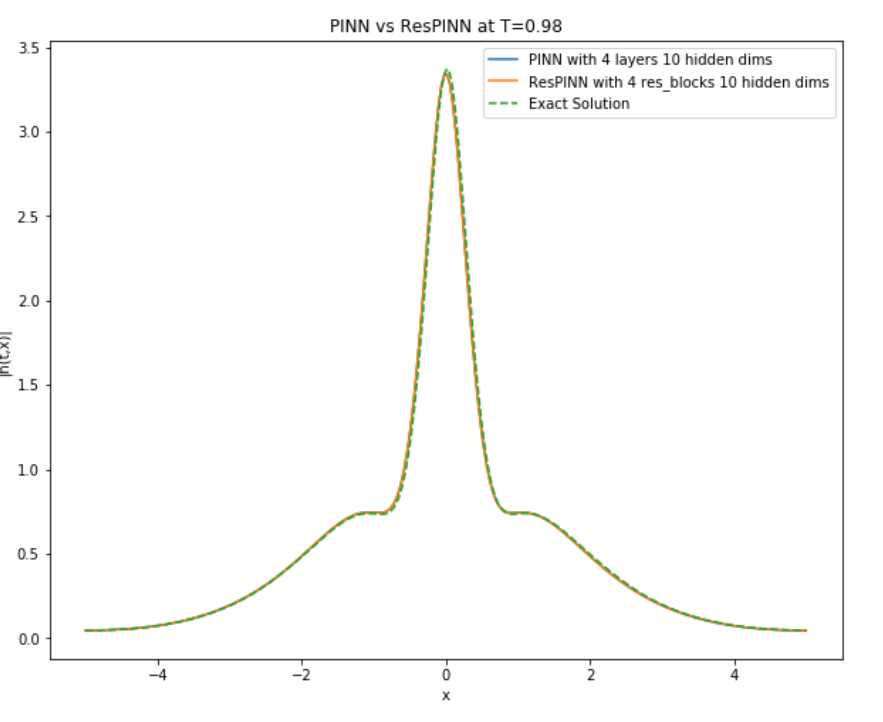
\includegraphics[height=4cm]{7.png}
    	\caption{解比较图}
    \end{figure}

   \subsection{比较不同隐藏层数对训练结果的影响}
   此处以ResPiNN网络框架作为基础网络来比较;dim\_hidden固定为50,并对比 res\_blocks=2, 4, 8 的loss曲线图和结果。
   \clearpage

   \begin{figure}
	\centering
	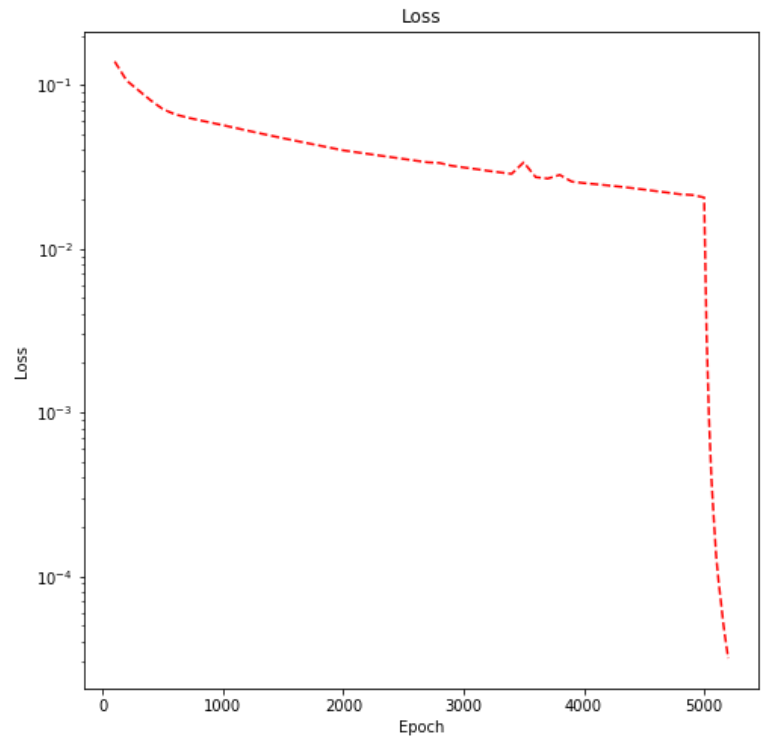
\includegraphics[height=4cm]{8.png}
	\caption{hidden\_layer=2; t=0.79}
   \end{figure}

   \begin{figure}
	\centering
	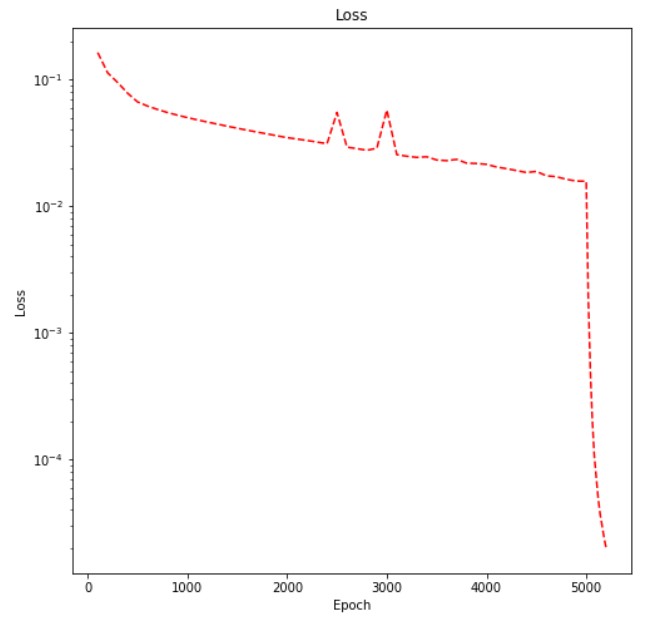
\includegraphics[height=4cm]{9.png}
	\caption{hidden\_layer=8; t=0.79}
	\end{figure}

   \begin{figure}
	\centering
	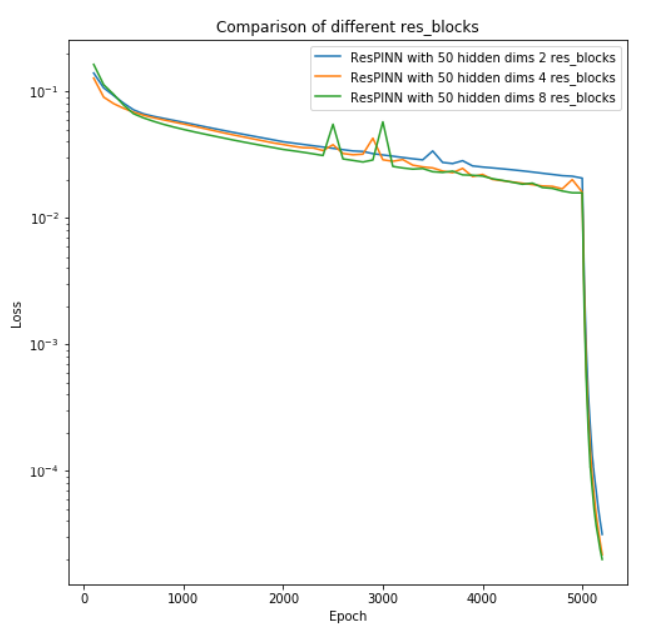
\includegraphics[height=4cm]{10.png}
	\caption{comparision of hidden\_layers; t=0.79}
	\end{figure}
	最后将已知的隐藏层是4的情况,将三条曲线放一起来做对比,由图像可以看到: 这三条loss曲线的下降都比较稳定,发现改变不同的res\_blocks对网络结果的影响并不大 并且为了追求效率,res\_blocks选为2就已经足够解决我们的问题
    
    \clearpage






\section{利用LSTM预测金融市场}

代码插入示例

\lstinputlisting{code/lstm.py} %花括号内为文件的路径

\end{document}
